\documentclass[11pt,a4paper]{article}

\usepackage[
    a4paper,
    left=15mm,
    right=15mm,
    top=30mm,
    bottom=25mm,
    headheight=25mm
]{geometry}
\usepackage{graphicx}
\usepackage{polski}
\usepackage[utf8]{inputenc}
\usepackage{enumerate}
\usepackage{comment}
\usepackage{fancyhdr}
\usepackage{hyperref}
\usepackage{indentfirst}
\usepackage{multirow}
\usepackage{multicol}
\usepackage{float}
\usepackage{amsmath}
\usepackage{amssymb}
\usepackage{wrapfig}
\usepackage{layout}
\usepackage{textcomp}
\usepackage[center]{caption}
\usepackage{subcaption}
\usepackage{siunitx}
\usepackage[mathscr]{euscript}
\usepackage{xcolor,colortbl}
\usepackage{setspace}
\usepackage{algorithm}
\usepackage[rightComments=false]{algpseudocodex}
\usepackage{listings}
\usepackage{amsthm}
\usepackage{needspace}

% no lone first/last lines of a paragraph on a page
\widowpenalty=10000
\clubpenalty=10000
\displaywidowpenalty=10000

\sisetup{output-exponent-marker=\ensuremath{\mathrm{e}}, output-decimal-marker={,}}
\algrenewcommand\algorithmicprocedure{\textbf{Procedura}}
\algrenewcommand\algorithmicfor{\textbf{Dla}}
\algrenewcommand\algorithmicdo{\textbf{powtarzaj}}
\algrenewcommand\algorithmicwhile{\textbf{Dopóki}}
\algrenewcommand\algorithmicloop{\textbf{Powtarzaj}}
\algrenewcommand\algorithmicif{\textbf{Jeżeli}}
\algrenewcommand\algorithmicelse{\textbf{Inaczej}}
\algrenewcommand\algorithmicthen{\textbf{wykonaj}}
\algrenewcommand\algorithmicend{\textbf{Koniec}}
\algrenewcommand\algorithmicreturn{\textbf{zwróć}}

\newenvironment{algorytm}[1][htb]
  {\par\bigskip\floatname{algorithm}{}\renewcommand{\thealgorithm}{}
   \begin{algorithm}[#1]%
  }{\end{algorithm}\par\bigskip}

\renewcommand{\baselinestretch}{1.18}
\renewcommand\thesubfigure{\roman{subfigure}}

\renewcommand\lstlistingname{Kod}
\lstset{
    language=Java,
    basicstyle=\ttfamily\footnotesize,
    keywordstyle=\bfseries,
    commentstyle=\itshape\color{gray},
    numbers=left,
    numberstyle=\tiny\color{gray},
    numbersep=8pt,
    frame=tb,
    xleftmargin=6mm,
    columns=fullflexible,
    keepspaces=true,
    showstringspaces=false,
    tabsize=4,
    captionpos=b,
    breaklines=true,
    postbreak=\mbox{\textcolor{gray}{$\hookrightarrow$}\space}
}

\pagestyle{fancy}
\fancyhead[L]{
    
\includegraphics[height=12mm]{img/agh-logo.jpg}
}
\fancyhead[R]{}

\author{Szymon Iwaniuk}
\title{
    
\includegraphics[height=45mm]{img/agh-logo.jpg}
    \vspace{10mm}
    \\
    Wzorce projektowe dla programowania współbieżnego}
\date{Teoria Współbieżności 2025/2026, laboratorium 7 \\ 23 listopada 2026}

\begin{document}

\maketitle
\tableofcontents
\pagebreak

\section{Wstęp}
\subsection{Treść zadania}
Zaimplementować bufor w problemie producentów i konsumentów jako aktywny obiekt (wzorzec
\textit{Active Object}). Wskazówki:
\begin{enumerate}
    \item Servant powinien implementować sam bufor i metody pomocnicze (np. sprawdzenie, czy bufor
          jest pusty lub pełny), bez żadnej logiki synchronizacji.
    \item Dla każdej metody aktywnego obiektu należy utworzyć podklasę \textit{Method Request}
          z metodą \texttt{guard()}, która sprawdza warunki synchronizacji przy użyciu metod Servanta.
    \item Proxy, tworzenie żądań i wstawianie ich do kolejki aktywacji wykonują się w wątku klienta,
          a Servant i Scheduler w osobnym, wspólnym wątku.
\end{enumerate}

\subsection{Wzorzec Active Object}
Active Object oddziela wywołanie metody od jej wykonania. Klient wywołuje metodę w swoim wątku
i od razu dostaje obiekt Future, a metoda wykonuje się później w wątku aktywnego obiektu.
Wzorzec składa się z sześciu elementów:
\begin{itemize}
    \item \textbf{Proxy} -- interfejs widoczny dla klientów. Wywołanie metody tworzy Method Request,
          wstawia je do kolejki aktywacji i zwraca Future.
    \item \textbf{Servant} -- implementacja obiektu (tu: bufor). Jego metody wywołuje wyłącznie
          Scheduler, w swoim wątku, więc Servant nie potrzebuje synchronizacji. Udostępnia też metody
          używane przez strażników.
    \item \textbf{Method Request} -- kontekst wywołania (parametry, Future) przekazywany z Proxy
          do Schedulera. Ma metodę \texttt{guard()} sprawdzającą, czy żądanie można wykonać,
          i \texttt{call()}, która wywołuje metodę Servanta.
    \item \textbf{Activation Queue} -- kolejka oczekujących żądań, zasób dzielony między wątki
          klientów (producenci żądań) i Scheduler (konsument żądań).
    \item \textbf{Scheduler} -- wątek, który zdejmuje żądania z kolejki i wykonuje te,
          których strażnik jest spełniony.
    \item \textbf{Future} -- miejsce na wynik. Klient odbiera wynik, gdy go potrzebuje,
          i blokuje się tylko wtedy, gdy żądanie nie zostało jeszcze wykonane.
\end{itemize}

\begin{figure}[H]
    \centering
    \begin{subfigure}{0.48\textwidth}
        \centering
        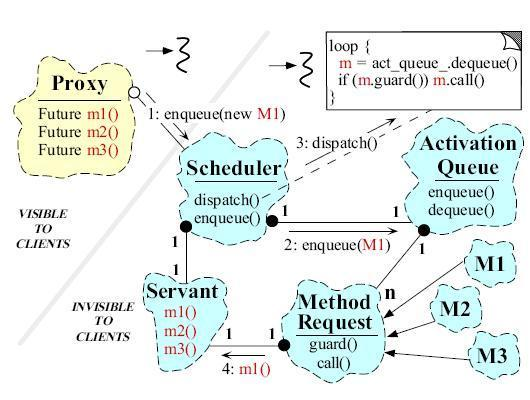
\includegraphics[width=\textwidth]{img/actobj-struct.jpg}
        \caption{Struktura}
    \end{subfigure}
    \hfill
    \begin{subfigure}{0.48\textwidth}
        \centering
        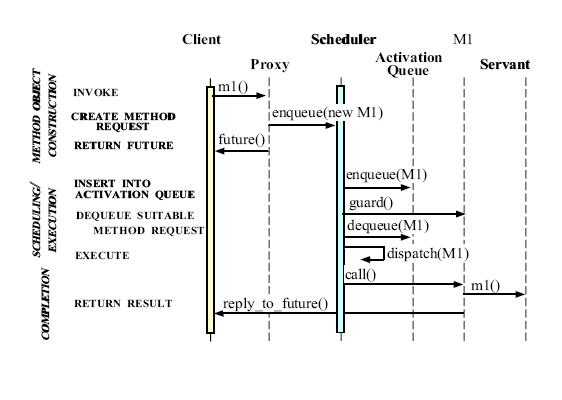
\includegraphics[width=\textwidth]{img/actobj-dynamic.jpg}
        \caption{Przebieg wywołania}
    \end{subfigure}
    \caption{Wzorzec Active Object (źródło: materiały do laboratorium)}
\end{figure}

\subsection{Opis rozwiązania}
Implementacja jest w języku \texttt{Java}. W porównaniu z przykładowym rozwiązaniem
z poprzedniego roku poprawiamy trzy rzeczy:
\begin{itemize}
    \item \textbf{Scheduler nie kręci się w pętli.} Żądanie, którego strażnik nie jest spełniony,
          nie wraca na koniec kolejki aktywacji (co powodowało aktywne czekanie i zmieniało kolejność
          żądań), tylko trafia do osobnej kolejki oczekujących żądań swojego typu. Gdy kolejka
          aktywacji jest pusta, Scheduler czeka na zmiennej warunkowej.
    \item \textbf{Proxy zwraca Future.} \texttt{put} zwraca \texttt{Future<Void>}, a \texttt{take}
          \texttt{Future<Integer>} z pobraną wartością, więc konsument rzeczywiście dostaje element.
    \item \textbf{Pomiary.} Porównujemy aktywny obiekt z buforem zrealizowanym jako monitor Javy
          i sprawdzamy, kiedy oddzielenie wywołania od wykonania się opłaca.
\end{itemize}
Razem ze sprawozdaniem zawarty jest pełny kod programu, program wykonujący pomiary
oraz skrypt generujący wykresy.

\section{Specyfikacja narzędzi i sprzętu}
Program został napisany w języku \texttt{Java 27} i uruchomiony na maszynie wirtualnej
\texttt{OpenJDK}, na komputerze z procesorem \texttt{Apple M4} (architektura \texttt{ARM64},
10 rdzeni: 4 wydajnościowe i 6 energooszczędnych), \texttt{16 GB} zunifikowanej pamięci
\texttt{LPDDR5} i systemem operacyjnym \texttt{macOS 26}.
Do wygenerowania wykresów użyty został \texttt{Python} z biblioteką \texttt{matplotlib}.

\subsection{Metoda pomiaru}
$p$ producentów i $p$ konsumentów przekazuje przez bufor łącznie $N = 20\,000$ elementów.
Każdy klient po każdym elemencie wykonuje własną pracę trwającą $w$ \textmu s, a każda operacja
na buforze (wstawienie, pobranie) kosztuje $s$ \textmu s, np. kopiowanie dużego obiektu.
Obie prace symulujemy aktywnym oczekiwaniem na \texttt{System.nanoTime()}, czyli zajmują procesor.
Porównujemy:
\begin{itemize}
    \item \textbf{Active Object} -- producent wywołuje \texttt{put}, wykonuje swoją pracę i dopiero
          wtedy czeka na Future. Konsument wywołuje \texttt{take}, wykonuje pracę i odbiera wartość,
    \item \textbf{monitor} -- metody \texttt{synchronized} z \texttt{wait()}/\texttt{notifyAll()};
          klient wykonuje pracę po powrocie z \texttt{put}/\texttt{take}. Operacja na buforze trwa
          wewnątrz sekcji krytycznej.
\end{itemize}
Parametry: $p \in \{1, 2, 4, 8\}$, rozmiar bufora $\in \{1, 10, 100\}$, $w \in \{0, 10, 100\}$ \textmu s,
$s \in \{0, 10\}$ \textmu s. Wszystkie wątki startują jednocześnie po zwolnieniu \texttt{CountDownLatch},
czas mierzymy \texttt{System.nanoTime()} do zakończenia ostatniego klienta. Po kilku przebiegach
rozgrzewających JIT każdą konfigurację uruchamiamy trzy razy i bierzemy medianę.
Po każdym przebiegu sprawdzamy, że konsumenci pobrali dokładnie $N$ elementów, a suma pobranych
wartości jest równa sumie wstawionych.

\section{Algorytmy}
\subsection{Proxy i Method Request}
Proxy działa w wątku klienta i nie wykonuje żadnej operacji na buforze -- tworzy tylko żądanie.

\begin{algorytm}[H]
\setstretch{1.4}
\begin{algorithmic}[1]
    \Procedure{put}{$x$} \Comment{wątek klienta}
        \State $r \gets$ \textsc{PutRequest}($x$), \ $r.\textit{future} \gets$ nowy Future
        \State \textit{activationQueue}.\Call{enqueue}{$r$}
        \State \Return $r.\textit{future}$
    \EndProcedure
    \Procedure{take}{} \Comment{wątek klienta}
        \State $r \gets$ \textsc{TakeRequest}(), \ $r.\textit{future} \gets$ nowy Future
        \State \textit{activationQueue}.\Call{enqueue}{$r$}
        \State \Return $r.\textit{future}$
    \EndProcedure
\end{algorithmic}
\caption{Proxy}
\end{algorytm}

Strażnicy korzystają wyłącznie z metod pomocniczych Servanta, a \textsc{call} wykonuje operację
i uzupełnia Future, budząc czekającego klienta.

\begin{algorytm}[H]
\setstretch{1.4}
\begin{algorithmic}[1]
    \Procedure{PutRequest.guard}{}
        \State \Return $\lnot$ \textit{servant}.\Call{isFull}{}
    \EndProcedure
    \Procedure{PutRequest.call}{}
        \State \textit{servant}.\Call{put}{$x$}, \ \textit{future}.\Call{set}{\texttt{null}}
    \EndProcedure
    \Procedure{TakeRequest.guard}{}
        \State \Return $\lnot$ \textit{servant}.\Call{isEmpty}{}
    \EndProcedure
    \Procedure{TakeRequest.call}{}
        \State \textit{future}.\Call{set}{\textit{servant}.\Call{take}{}}
    \EndProcedure
\end{algorithmic}
\caption{Strażnicy i wykonanie żądań}
\end{algorytm}

\subsection{Scheduler}
\begin{algorytm}[H]
\setstretch{1.4}
\begin{algorithmic}[1]
    \Procedure{scheduler}{} \Comment{osobny wątek, jedyny używający Servanta}
        \Loop
            \If{$P \ne \emptyset \land$ \Call{first}{$P$}.\Call{guard}{}}
                \State \Call{removeFirst}{$P$}.\Call{call}{}
            \ElsIf{$T \ne \emptyset \land$ \Call{first}{$T$}.\Call{guard}{}}
                \State \Call{removeFirst}{$T$}.\Call{call}{}
            \Else
                \State $r \gets$ \textit{activationQueue}.\Call{dequeue}{} \Comment{czeka, gdy kolejka jest pusta}
                \State $Q \gets$ \textbf{jeżeli} $r$ to \textsc{PutRequest} \textbf{to} $P$ \textbf{inaczej} $T$
                \If{$Q = \emptyset \land r.$\Call{guard}{}}
                    \State $r.$\Call{call}{}
                \Else
                    \State dopisz $r$ na koniec $Q$
                \EndIf
            \EndIf
        \EndLoop
    \EndProcedure
\end{algorithmic}
\caption{Pętla Schedulera; $P$, $T$ -- kolejki oczekujących wstawień i pobrań}
\end{algorytm}

Scheduler najpierw sprawdza, czy wykonanie poprzedniego żądania nie odblokowało pierwszego
oczekującego wstawienia lub pobrania (wiersze 3--6). Nowe żądanie wykonuje od razu tylko wtedy,
gdy nie czeka przed nim żadne żądanie tego samego typu (wiersz 10), więc wstawienia i pobrania
są wykonywane w kolejności nadejścia. Nie może dojść do sytuacji, w której obie kolejki
oczekujących są niepuste i żadne żądanie nie może być wykonane: wstawienie czeka tylko przy pełnym
buforze, a wtedy każde pobranie jest wykonalne, i odwrotnie. Gdy obie kolejki są puste albo ich
pierwsze żądania nie są wykonalne, Scheduler blokuje się w \textsc{dequeue} na zmiennej warunkowej
zamiast aktywnie czekać.

\section{Implementacja}
Poniżej znajdują się najważniejsze klasy. Pełny kod (w tym klasy \textbf{Servant},
\textbf{MonitorBuffer} i program pomiarowy \textbf{Main}) jest w katalogu \texttt{src} dołączonym do sprawozdania.

\begin{lstlisting}[caption={Klasa \textbf{Proxy} (\texttt{src/Proxy.java})}]
/** Proxy: interface for clients, runs in the client thread, returns futures immediately. */
class Proxy {
    private final Servant servant;
    private final ActivationQueue queue;

    Proxy(Servant servant, ActivationQueue queue) {
        this.servant = servant;
        this.queue = queue;
    }

    Future<Void> put(int value) {
        PutRequest r = new PutRequest(servant, value);
        queue.enqueue(r);
        return r.future;
    }

    Future<Integer> take() {
        TakeRequest r = new TakeRequest(servant);
        queue.enqueue(r);
        return r.future;
    }
}
\end{lstlisting}

\begin{lstlisting}[caption={Klasy \textbf{MethodRequest}, \textbf{PutRequest}, \textbf{TakeRequest} (\texttt{src/MethodRequest.java})}]
/** Method Request: call context passed from the proxy to the scheduler. */
abstract class MethodRequest {
    protected final Servant servant;

    MethodRequest(Servant servant) {
        this.servant = servant;
    }

    /** Synchronization condition, checked by the scheduler before call(). */
    abstract boolean guard();

    abstract void call();
}

class PutRequest extends MethodRequest {
    private final int value;
    final Future<Void> future = new Future<>();

    PutRequest(Servant servant, int value) {
        super(servant);
        this.value = value;
    }

    @Override
    boolean guard() {
        return !servant.isFull();
    }

    @Override
    void call() {
        servant.put(value);
        future.set(null);
    }
}

class TakeRequest extends MethodRequest {
    final Future<Integer> future = new Future<>();

    TakeRequest(Servant servant) {
        super(servant);
    }

    @Override
    boolean guard() {
        return !servant.isEmpty();
    }

    @Override
    void call() {
        future.set(servant.take());
    }
}
\end{lstlisting}

\begin{lstlisting}[caption={Klasa \textbf{ActivationQueue} (\texttt{src/ActivationQueue.java})}]
import java.util.ArrayDeque;
import java.util.concurrent.locks.Condition;
import java.util.concurrent.locks.ReentrantLock;

/** Activation Queue: FIFO of method requests, clients enqueue, the scheduler dequeues. */
class ActivationQueue {
    private final ArrayDeque<MethodRequest> queue = new ArrayDeque<>();
    private final ReentrantLock lock = new ReentrantLock();
    private final Condition notEmpty = lock.newCondition();

    void enqueue(MethodRequest r) {
        lock.lock();
        try {
            queue.addLast(r);
            notEmpty.signal();
        } finally {
            lock.unlock();
        }
    }

    MethodRequest dequeue() throws InterruptedException {
        lock.lock();
        try {
            while (queue.isEmpty()) notEmpty.await();
            return queue.pollFirst();
        } finally {
            lock.unlock();
        }
    }
}
\end{lstlisting}

\begin{lstlisting}[caption={Klasa \textbf{Scheduler} (\texttt{src/Scheduler.java})}]
import java.util.ArrayDeque;

/**
 * Scheduler: its own thread, the only one that touches the servant. A request whose guard fails
 * goes to the waiting queue of its type instead of back to the activation queue, so the scheduler
 * never spins and requests of one type are executed in arrival order.
 */
class Scheduler extends Thread {
    private final ActivationQueue queue;
    private final ArrayDeque<MethodRequest> waitingPuts = new ArrayDeque<>();
    private final ArrayDeque<MethodRequest> waitingTakes = new ArrayDeque<>();
    private volatile boolean running = true;

    Scheduler(ActivationQueue queue) {
        this.queue = queue;
    }

    void shutdown() {
        running = false;
        interrupt();
    }

    @Override
    public void run() {
        try {
            while (running) {
                // a call may have made the head of a waiting queue executable
                if (!waitingPuts.isEmpty() && waitingPuts.peekFirst().guard()) {
                    waitingPuts.pollFirst().call();
                } else if (!waitingTakes.isEmpty() && waitingTakes.peekFirst().guard()) {
                    waitingTakes.pollFirst().call();
                } else {
                    MethodRequest r = queue.dequeue();
                    ArrayDeque<MethodRequest> waiting = r instanceof PutRequest ? waitingPuts : waitingTakes;
                    if (waiting.isEmpty() && r.guard()) r.call();
                    else waiting.addLast(r); // keep FIFO behind earlier requests of this type
                }
            }
        } catch (InterruptedException e) {
            // shutdown
        }
    }
}
\end{lstlisting}

\begin{lstlisting}[caption={Klasa \textbf{Future} (\texttt{src/Future.java})}]
/** Future: placeholder for the result, filled by the scheduler thread, read by the client. */
class Future<T> {
    private T value;
    private boolean done = false;

    synchronized void set(T v) {
        value = v;
        done = true;
        notifyAll();
    }

    synchronized boolean isDone() {
        return done;
    }

    synchronized T get() throws InterruptedException {
        while (!done) wait();
        return value;
    }
}
\end{lstlisting}

\section{Wyniki}
\subsection{Tani bufor ($s = 0$)}
\textbf{Rysunek 2} pokazuje czas przekazania wszystkich elementów, gdy operacja na buforze
nic nie kosztuje. Linie ciągłe to aktywny obiekt, przerywane -- monitor. Kolor oznacza rozmiar bufora.

\begin{figure}[H]
    \centering
    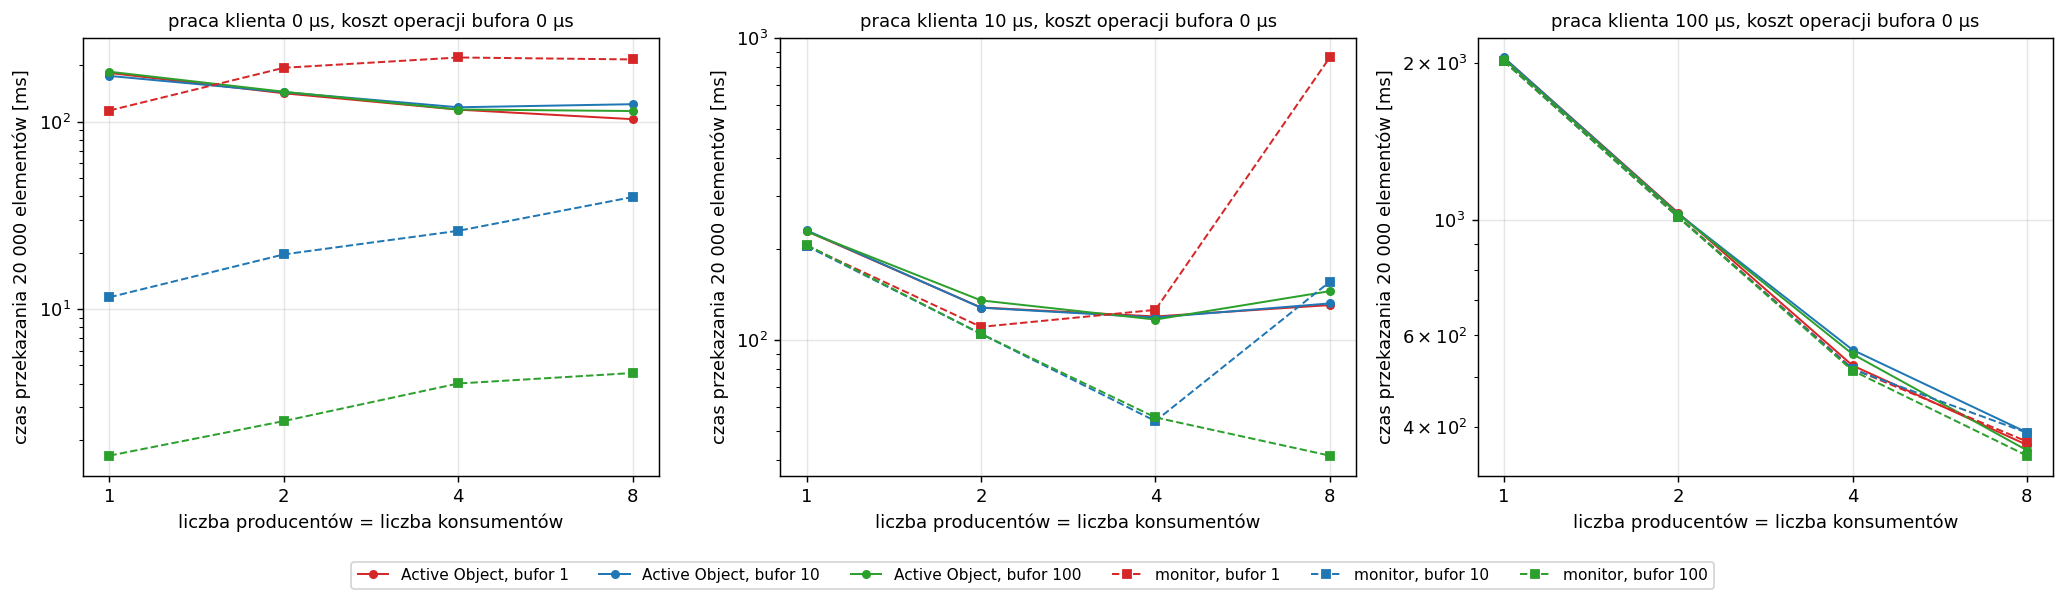
\includegraphics[width=\textwidth]{img/times_s0.png}
    \caption{Czas wykonania, koszt operacji na buforze $s = 0$}
\end{figure}

Bez pracy klientów ($w = 0$) aktywny obiekt jest bardzo wolny: przekazanie $20\,000$ elementów
trwa 114--185 ms, podczas gdy monitor z buforem 100 potrzebuje 1,6--4,6 ms (25--112 razy mniej).
Każde wywołanie to utworzenie żądania i Future, wstawienie do kolejki pod blokadą,
przełączenie do wątku Schedulera i obudzenie klienta czekającego na Future -- łącznie 2,9--4,6 \textmu s
na żądanie. Wszystkie żądania wykonuje jeden wątek, więc ten koszt jest sumowany, a czas aktywnego
obiektu prawie nie zależy od rozmiaru bufora ani liczby klientów. Wyjątkiem jest bufor o rozmiarze 1:
monitor musi przy każdym elemencie budzić drugą stronę i zwalnia z 115 ms ($p = 1$) do 216 ms ($p = 8$),
a aktywny obiekt dla $p \ge 2$ jest od niego szybszy (103--142 ms).

Przy pracy $w = 10$ \textmu s monitor z dużym buforem skaluje się z liczbą wątków (207 ms dla $p = 1$,
41 ms dla $p = 8$), a aktywny obiekt dla $p \ge 2$ zatrzymuje się na około 117--145 ms -- tyle trwa obsłużenie
$40\,000$ żądań przez jeden wątek Schedulera, który staje się wąskim gardłem. Z drugiej strony
monitor z buforem 1 i $p = 8$ potrzebuje aż 862 ms, bo 16 wątków wykonujących aktywną pracę
na 10 rdzeniach rywalizuje o jeden monitor, a \texttt{notifyAll()} budzi wszystkich czekających;
aktywny obiekt w tej samej konfiguracji potrzebuje 131 ms.
Przy $w = 100$ \textmu s czas obu rozwiązań różni się o najwyżej 9\% i jest bliski czasowi samej pracy
klienta ($N \cdot w / p$, np. 2000 ms dla $p = 1$): synchronizacja przestaje mieć znaczenie.

\subsection{Kosztowny bufor ($s = 10$ \textmu s)}
\textbf{Rysunek 3} pokazuje te same pomiary, gdy każda operacja na buforze kosztuje 10 \textmu s.
Operacje na buforze zawsze wykonują się po kolei, więc czas nie może być krótszy niż
$2 N s = 400$ ms.

\begin{figure}[H]
    \centering
    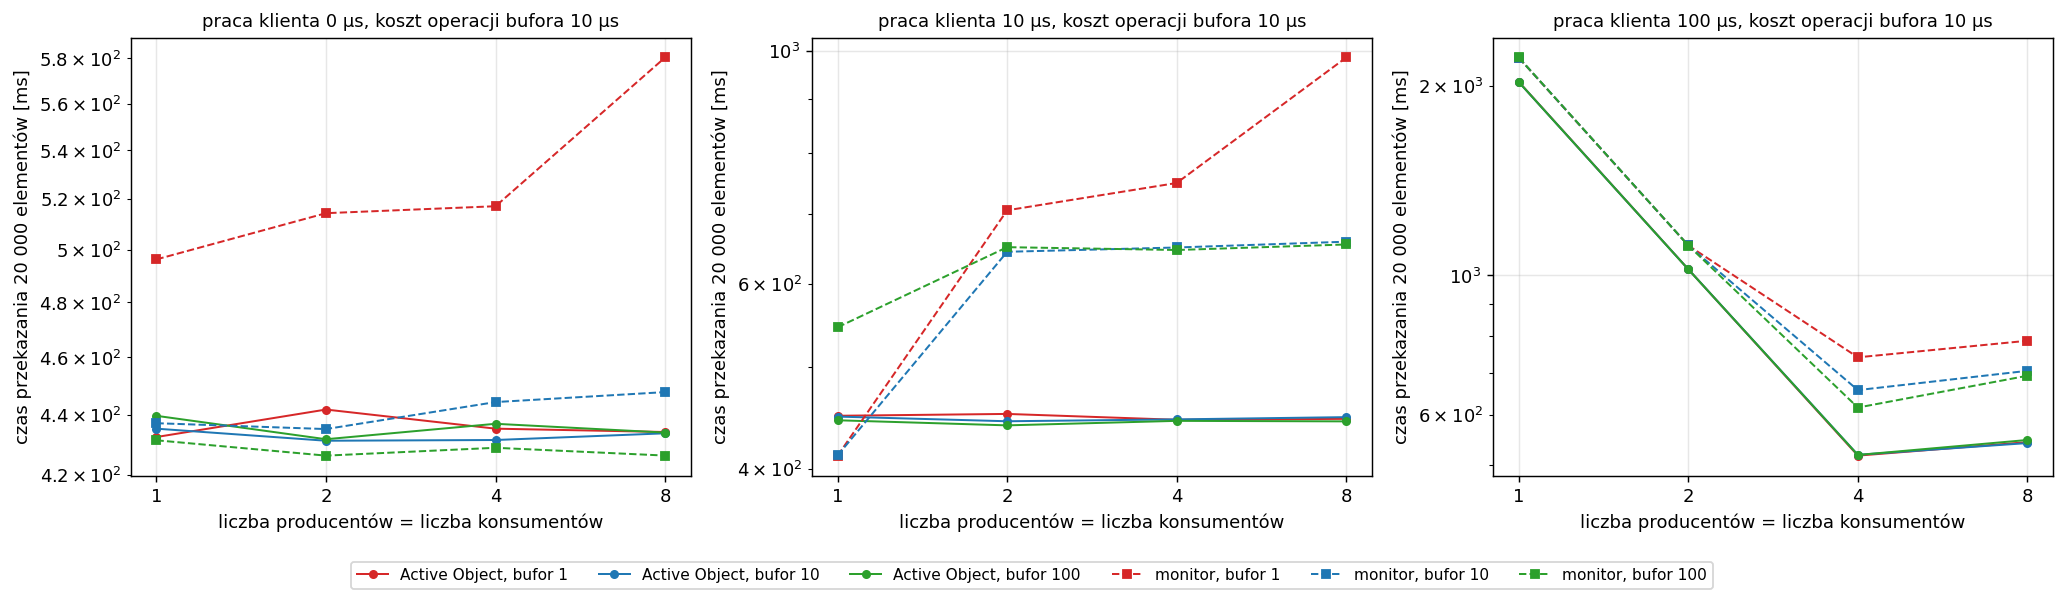
\includegraphics[width=\textwidth]{img/times_s10.png}
    \caption{Czas wykonania, koszt operacji na buforze $s = 10$ \textmu s}
\end{figure}

Tu aktywny obiekt wygrywa. Dla $w \le 10$ \textmu s jego czas wynosi 431--451 ms niezależnie
od liczby klientów i rozmiaru bufora, czyli jest bliski dolnej granicy 400 ms: Scheduler wykonuje
operacje jedna po drugiej, a klienci w tym czasie wykonują swoją pracę. W monitorze klient czeka
na wejście do sekcji krytycznej, w której inny klient wykonuje kosztowną operację, a dopiero potem
wykonuje własną pracę. Dla $w = 10$ \textmu s i $p \ge 2$ monitor potrzebuje 644--986 ms,
czyli aktywny obiekt jest od niego o 31--55\% szybszy. Przy $w = 100$ \textmu s i $p = 1$ monitor
potrzebuje 2218--2220 ms, co odpowiada sumie $N(w + s) = 2200$ ms, a aktywny obiekt 2029--2031 ms,
bo operacja na buforze wykonuje się w czasie pracy klienta. Dla $p = 8$ jest to 541--547 ms wobec
692--787 ms. Monitor był szybszy tylko bez pracy klientów ($w = 0$, o 1--2\%, gdy oba rozwiązania są ograniczone
przez kolejne operacje na buforze) oraz dla jednego producenta i jednego konsumenta przy $w = 10$ \textmu s
i buforze 1 lub 10 (412 ms wobec 448--449 ms), gdy nie ma rywalizacji o monitor.

\textbf{Tabela 1} zestawia mediany dla bufora o rozmiarze 10.

\begin{table}[H]
    \centering
    \renewcommand{\arraystretch}{1.3}
    \begin{tabular}{|r|r|r|r|r|r|r|r|r|r|}
        \hline
        \multirow{2}{*}{$s$ [\textmu s]} & \multirow{2}{*}{$w$ [\textmu s]} & \multicolumn{4}{c|}{Active Object [ms]} & \multicolumn{4}{c|}{monitor [ms]} \\ \cline{3-10}
        & & $p = 1$ & $p = 2$ & $p = 4$ & $p = 8$ & $p = 1$ & $p = 2$ & $p = 4$ & $p = 8$ \\ \hline
        0 & 0 & \num{175.9} & \num{144.1} & \num{119.6} & \num{124.2} & \num{11.6} & \num{19.6} & \num{26.2} & \num{39.7} \\
        0 & 10 & \num{230.7} & \num{127.9} & \num{118.7} & \num{132.2} & \num{204.9} & \num{104.8} & \num{53.9} & \num{155.8} \\
        0 & 100 & \num{2048.3} & \num{1026.9} & \num{562.6} & \num{390.5} & \num{2017.1} & \num{1012.1} & \num{516.4} & \num{390.1} \\ \hline
        10 & 0 & \num{435.3} & \num{431.2} & \num{431.5} & \num{433.7} & \num{437.1} & \num{435.2} & \num{444.4} & \num{447.8} \\
        10 & 10 & \num{448.3} & \num{443.8} & \num{445.6} & \num{447.8} & \num{411.7} & \num{643.7} & \num{649.8} & \num{658.2} \\
        10 & 100 & \num{2029.3} & \num{1022.3} & \num{518.3} & \num{541.1} & \num{2219.2} & \num{1115.5} & \num{656.9} & \num{704.9} \\ \hline
    \end{tabular}
    \caption{Czas przekazania $20\,000$ elementów, bufor o rozmiarze 10}
\end{table}

\section{Wnioski}
Wzorzec Active Object oddziela wywołanie metody od jej wykonania: Proxy w wątku klienta tylko
tworzy żądanie, a jedyny wątek Schedulera wykonuje operacje na Servancie, więc Servant nie potrzebuje
żadnej synchronizacji, a warunki synchronizacji są zapisane jawnie w strażnikach.
Dzięki kolejkom oczekujących żądań Scheduler nie czeka aktywnie i wykonuje żądania tego samego
typu w kolejności nadejścia, czego nie zapewniało ponowne wstawianie żądania do kolejki aktywacji.

Wydajność zależy od stosunku kosztu operacji na obiekcie do narzutu wzorca, który w naszej implementacji
wynosi 3--5 \textmu s na żądanie. Gdy operacja na buforze jest tania, aktywny obiekt jest wielokrotnie
wolniejszy od monitora, a jeden wątek Schedulera ogranicza przepustowość. Gdy operacja jest kosztowna,
a klienci mają własną pracę, aktywny obiekt jest zwykle szybszy o 8--55\%, bo klient wykonuje swoją pracę
w czasie, gdy Scheduler realizuje jego żądanie, i nie rywalizuje o blokadę z innymi klientami.
Wzorzec opłaca się więc dla obiektów z kosztownymi operacjami, np. dostępem do urządzeń lub sieci,
a nie dla prostych struktur danych.

\begin{thebibliography}{9}
    \bibitem{schmidt} R.G. Lavender, D.C. Schmidt: \textit{Active Object -- An Object Behavioral Pattern for Concurrent Programming}. \url{https://www.dre.vanderbilt.edu/~schmidt/PDF/Active-Objects.pdf}
    \bibitem{agh} \url{https://home.agh.edu.pl/~funika/tw/lab7/}
    \bibitem{wzorce} \url{https://home.agh.edu.pl/~funika/tw/lab7/TW-wzorce.pdf}
\end{thebibliography}

\end{document}

